%=======================================================================
%  Laboratorio N.o 1 - Circuitos Electronicos
%  UCSP - Facultad de Ingenieria - Ing. Electronica y de Telecomunicaciones
%  Transcripcion a LaTeX del documento "Laboratorio_1_Propedeucio EEB.doc"
%  Compilar con:  pdflatex Laboratorio_1.tex   (dos veces)
%=======================================================================
\documentclass[11pt,a4paper]{article}

\usepackage[utf8]{inputenc}
\usepackage[T1]{fontenc}
\usepackage[spanish,es-nodecimaldot]{babel}
\usepackage{lmodern}

\usepackage[left=2.5cm,right=2.5cm,top=3cm,bottom=2.5cm,headheight=28pt]{geometry}
\usepackage{graphicx}
\usepackage{float}
\usepackage{caption}
\usepackage{enumitem}
\usepackage{array}
\usepackage{tabularx}
\usepackage{multirow}
\usepackage{amsmath,amssymb}
\usepackage{textcomp}
\usepackage{fancyhdr}
\usepackage{xcolor}
\usepackage[hidelinks]{hyperref}

% ---------------------------------------------------------------- rutas
\graphicspath{{imagenes/}}

% ------------------------------------------------------------ encabezado
\pagestyle{fancy}
\fancyhf{}
\fancyhead[L]{\footnotesize UCSP -- Facultad de Ingeniería\\ Ing. Electrónica y de Telecomunicaciones}
\fancyhead[R]{\footnotesize 2026-2 Circuitos Electrónicos\\ Ebert San Román Castillo}
\fancyfoot[C]{\thepage}
\renewcommand{\headrulewidth}{0.4pt}

% ------------------------------------------------------------- comandos
\newcommand{\linearesp}{\noindent\rule{\linewidth}{0.4pt}\\[10pt]}
\captionsetup{font=small,labelfont=bf}
\setlist[itemize]{itemsep=2pt,topsep=4pt}
\setlist[enumerate]{itemsep=6pt,topsep=4pt}

\begin{document}

%=======================================================================
%  CABECERA DE LA GUIA
%=======================================================================
\begin{center}
    {\Large\bfseries PRIMERA UNIDAD: MI PRIMER CIRCUITO}
\end{center}

\vspace{0.4cm}

\renewcommand{\arraystretch}{1.5}
\noindent
\begin{tabularx}{\textwidth}{|c|X|c|}
\hline
\multirow{2}{*}{\Huge\bfseries 1} & \centering\bfseries Guía de Prácticas & \multirow{2}{*}{\parbox{2.2cm}{\centering\bfseries Nota\\[1.2cm]}}\\
\cline{2-2}
 & \centering\arraybackslash\bfseries Mi primer Circuito de Electrónica & \\
\hline
\multicolumn{3}{|l|}{\textbf{Grupo:} \rule{4cm}{0.4pt}}\\
\hline
\multicolumn{3}{|l|}{\textbf{Alumno(s):} \rule{11cm}{0.4pt}}\\
\multicolumn{3}{|l|}{\phantom{\textbf{Alumno(s):}} \rule{11cm}{0.4pt}}\\
\hline
\end{tabularx}
\renewcommand{\arraystretch}{1}

\vspace{0.8cm}

%=======================================================================
\section*{I.\quad Objetivos}

\begin{itemize}
    \item Aprender a utilizar el sistema de medición \emph{Electronic Explorer Board}.
    \item Reconocer las formas de las señales analógicas gráficamente.
    \item Ver las herramientas y utilidades que posee el software, en particular los conceptos
          básicos de los equipos de instrumentación en electrónica, como lo son fuentes,
          generadores y osciloscopios.
    \item Reconocer componentes electrónicos tales como el diodo LED, resistencia,
          potenciómetro y display de 7 segmentos.
    \item Introducción básica a las leyes fundamentales de la electrónica: la ley de Ohm.
\end{itemize}

%=======================================================================
\section*{II.\quad Contenido teórico}

\subsection*{Capítulo 1: La Electrónica}

La electrónica es la rama de la física y especialización de la ingeniería, que estudia y emplea
sistemas cuyo funcionamiento se basa en la conducción y el control del flujo de los electrones
u otras partículas cargadas eléctricamente, consiguiendo múltiples aplicaciones como por ejemplo,
la radio, la televisión, los equipos de sonido, los ordenadores, los robots, la automatización
industrial, los sistemas de control y gestión del automóvil y los equipos de medida, etc.

La electrónica se puede dividir en 2 grandes ramas:

\begin{itemize}
    \item La electrónica analógica.
    \item La electrónica digital.
\end{itemize}

En la figura~\ref{fig:audio} se describen 2 procesos de sistemas electrónicos de audio, tanto de
señal analógica como de señal digital.

\begin{figure}[H]
    \centering
    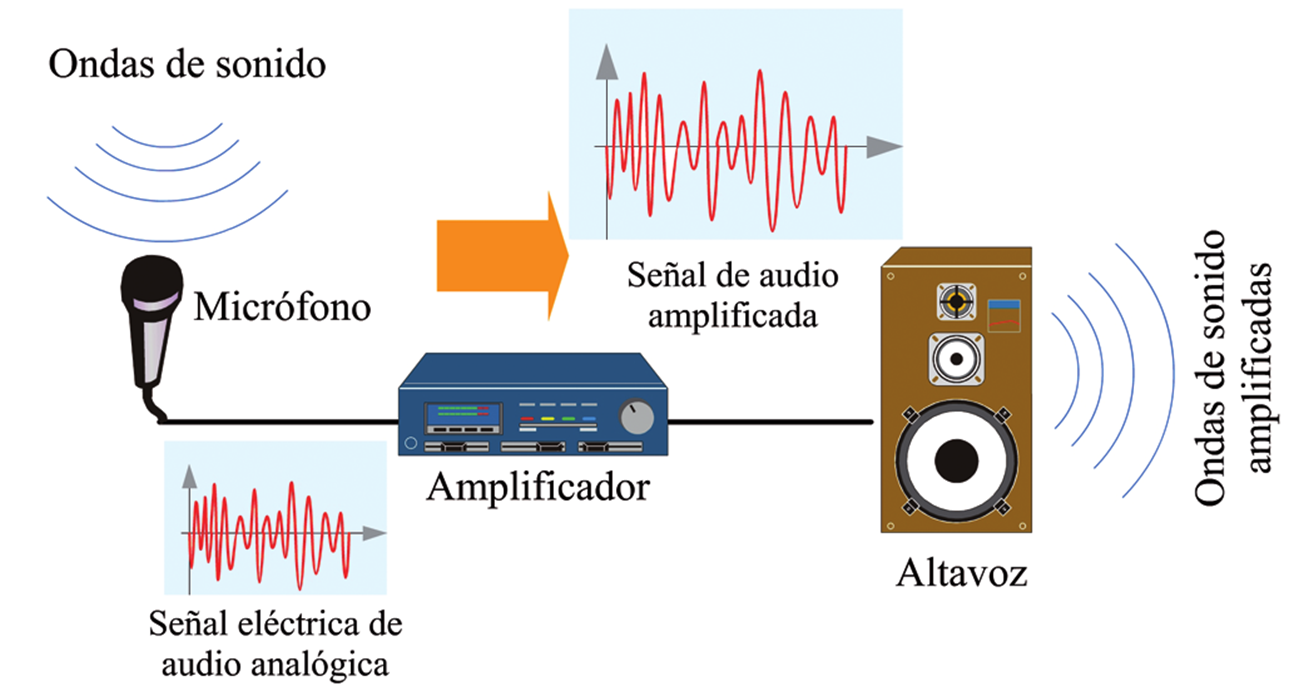
\includegraphics[width=0.85\textwidth]{image01.png}\\[6pt]
    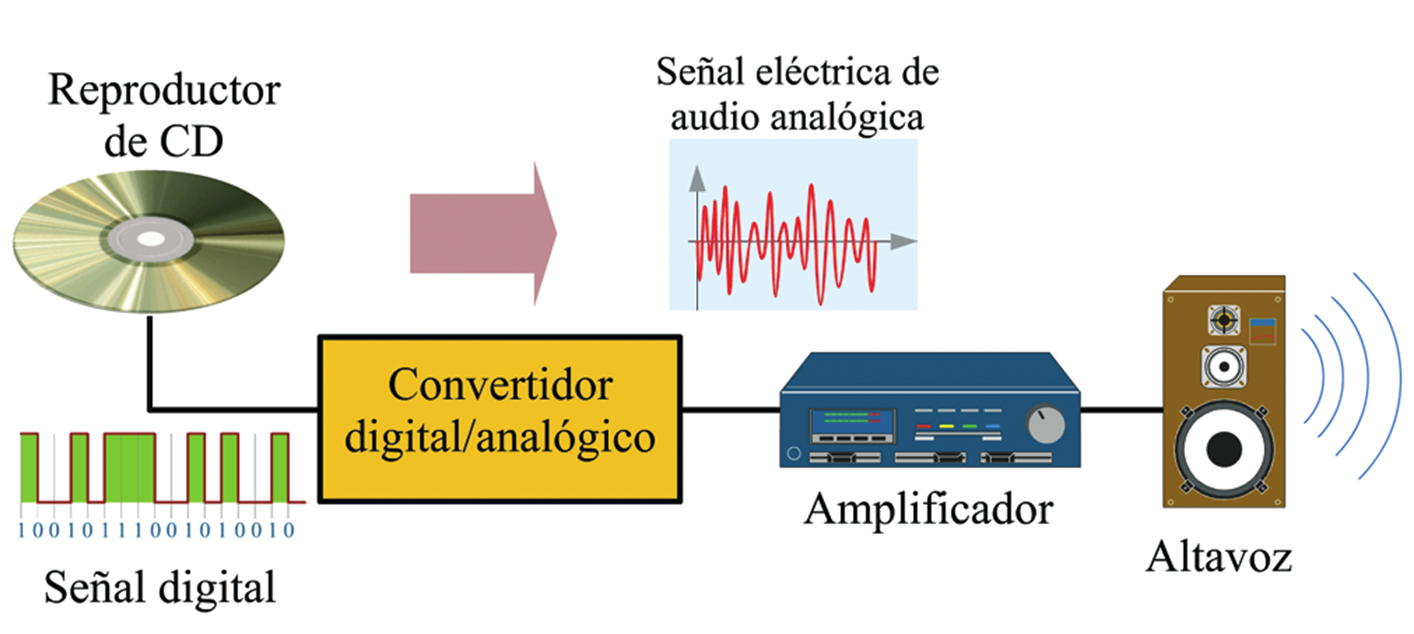
\includegraphics[width=0.85\textwidth]{image02.png}
    \caption{Sistema de Audio con procesamiento analógico y digital.}
    \label{fig:audio}
\end{figure}

El movimiento de electrones que se establece en un conductor se llama corriente $i(t)$; la
corriente puede ser corriente continua (CC -- DC) o corriente alterna (CA -- AC) como se aprecia
en la figura~\ref{fig:cacc}. La unidad de la corriente es el Ampere (A).

\begin{figure}[H]
    \centering
    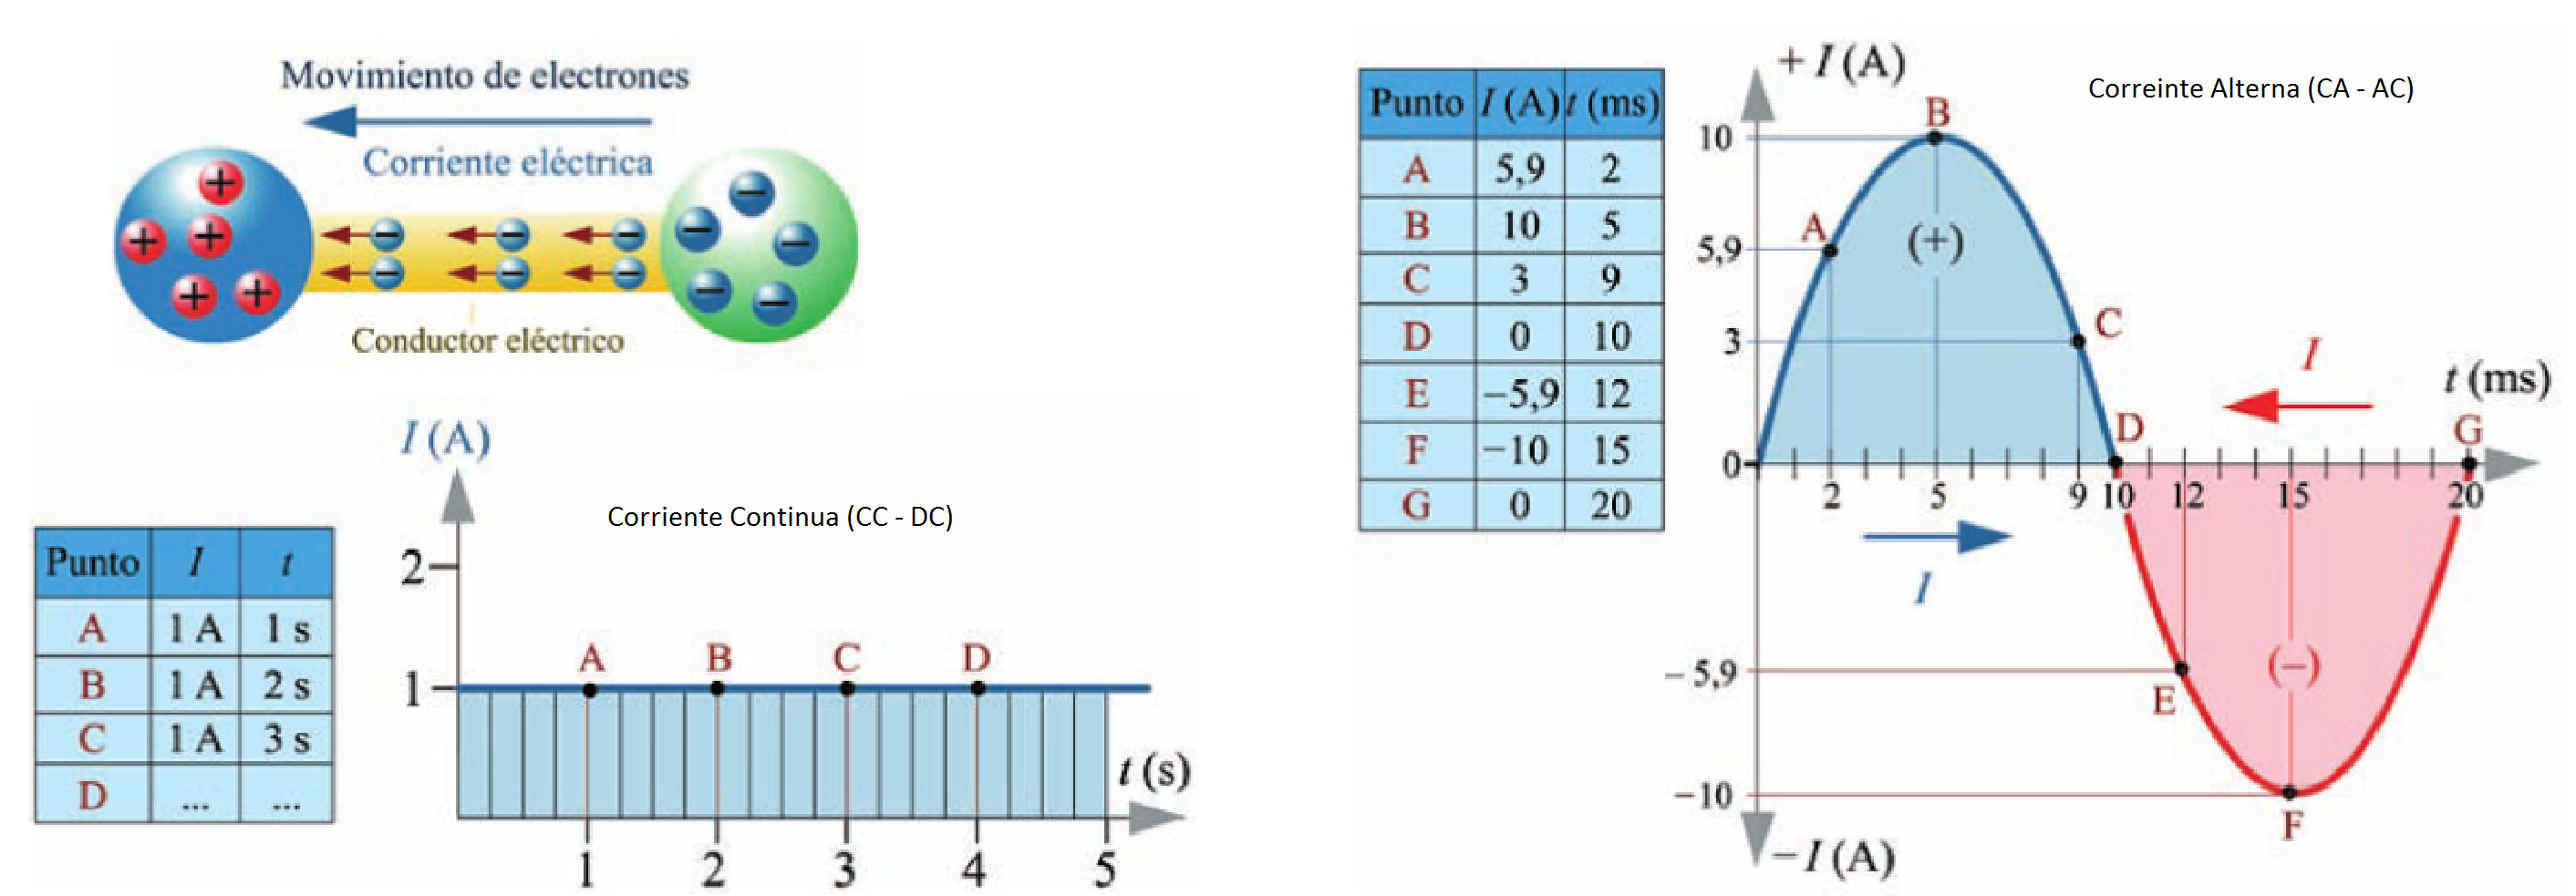
\includegraphics[width=0.9\textwidth]{image03.png}
    \caption{Corriente alterna vs corriente continua.}
    \label{fig:cacc}
\end{figure}

Para generar una corriente es necesario que aparezca una fuerza capaz de mover los electrones
libres del circuito, que se denomina FEM (Fuerza Electromotriz -- Fuente), ver
figura~\ref{fig:fuente}, que genera una tensión eléctrica o diferencia de potencial (también
denominada voltaje $V$), que es una magnitud física que cuantifica la diferencia de potencial
eléctrico entre dos puntos. Su unidad de medida es el voltio (V).

\begin{figure}[H]
    \centering
    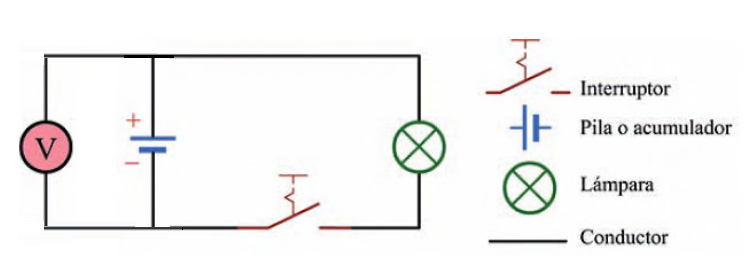
\includegraphics[width=0.55\textwidth]{image04.png}
    \caption{Fuente de Tensión (Voltaje) en un circuito eléctrico.}
    \label{fig:fuente}
\end{figure}

Un circuito eléctrico está compuesto por conductores y aislantes; los conductores permiten el
paso de corriente con facilidad, mientras que los aislantes bloquean el paso de la corriente.
En la figura~\ref{fig:cable} podemos observar la constitución de los cables eléctricos que
utilizaremos en la práctica, el cual está formado por un cable metálico de cobre (conductor) y un
recubrimiento de plástico (aislante), que evita que la corriente fugue a otro lugar no deseado.

\begin{figure}[H]
    \centering
    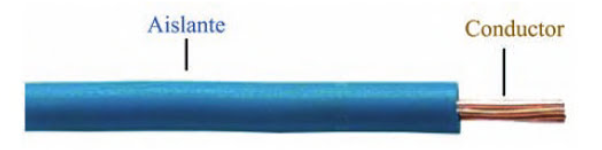
\includegraphics[width=0.55\textwidth]{image05.png}
    \caption{Partes de un cable eléctrico.}
    \label{fig:cable}
\end{figure}

La resistencia eléctrica es una medida de la cantidad de oposición que ofrecen los cuerpos al
paso de la corriente. Su unidad de medida es el Ohmio y está representada por la letra griega
omega $\Omega$; los esquemáticos y modelos de las resistencias se pueden ver en la
figura~\ref{fig:resist}.

\begin{figure}[H]
    \centering
    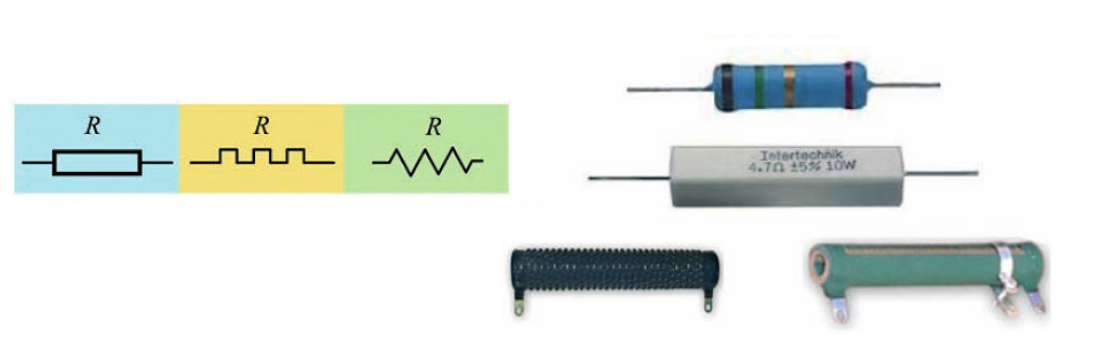
\includegraphics[width=0.8\textwidth]{image06.png}
    \caption{Símbolos y modelos de resistencias eléctricas.}
    \label{fig:resist}
\end{figure}

El físico alemán Ohm, mediante un experimento, descubrió que la intensidad de corriente que
recorre un circuito eléctrico es directamente proporcional a la tensión aplicada e inversamente
proporcional a la resistencia eléctrica, como se puede ver en la figura~\ref{fig:ohm}.

\begin{equation}
    I = \frac{V}{R}
    \qquad\Longleftrightarrow\qquad
    V = I\,R
    \qquad\Longleftrightarrow\qquad
    R = \frac{V}{I}
\end{equation}

\begin{figure}[H]
    \centering
    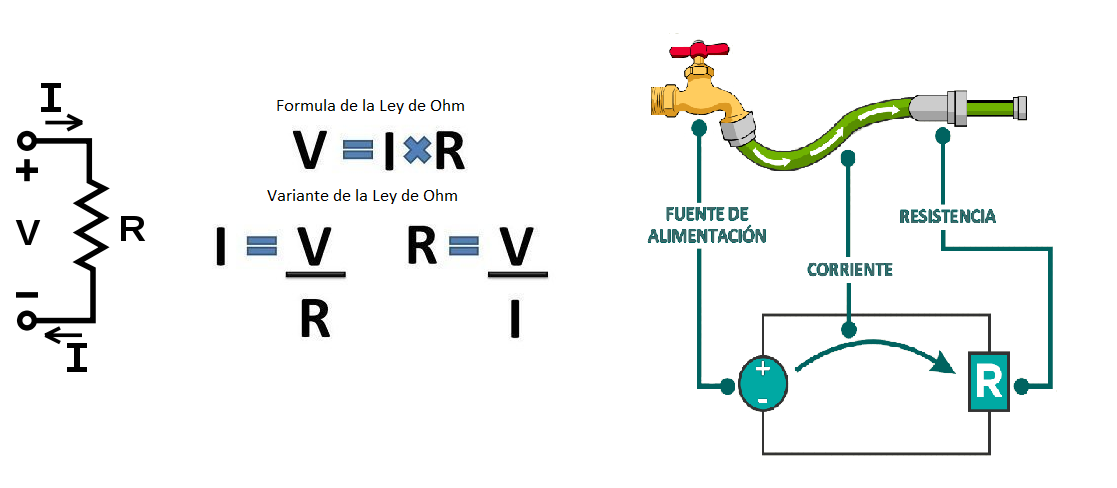
\includegraphics[width=0.75\textwidth]{image07.png}
    \caption{La Ley de Ohm y su interpretación.}
    \label{fig:ohm}
\end{figure}

Las resistencias se fabrican con diferentes valores óhmicos, pero es muy difícil fabricar una
resistencia con un valor exacto; mientras más exacta sea la resistencia más se encarece el precio
del producto, de aquí nace el concepto de \textbf{tolerancia}, que indica los valores máximo y
mínimo de la resistencia.

Para entender mejor la exactitud de la resistencia, en la figura~\ref{fig:carbon} se aprecia el
modelo de resistencia de carbón, que es la más usada para pequeñas potencias. La resistencia
consiste en un cilindro aislado en el que se deposita una película delgada de carbón entre 2
conductores metálicos en los extremos; para obtener una resistencia determinada se realiza una
excavación helicoidal a lo largo de la película de carbón.

\begin{figure}[H]
    \centering
    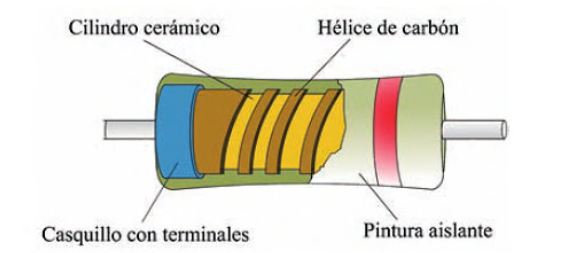
\includegraphics[width=0.5\textwidth]{image08.png}
    \caption{Resistencia de película de carbón.}
    \label{fig:carbon}
\end{figure}

Los valores comerciales de las resistencias se representan a través de una serie de anillos de
colores pintados sobre la superficie esmaltada de la resistencia, que se leen de acuerdo a la
figura~\ref{fig:colores}.

\begin{figure}[H]
    \centering
    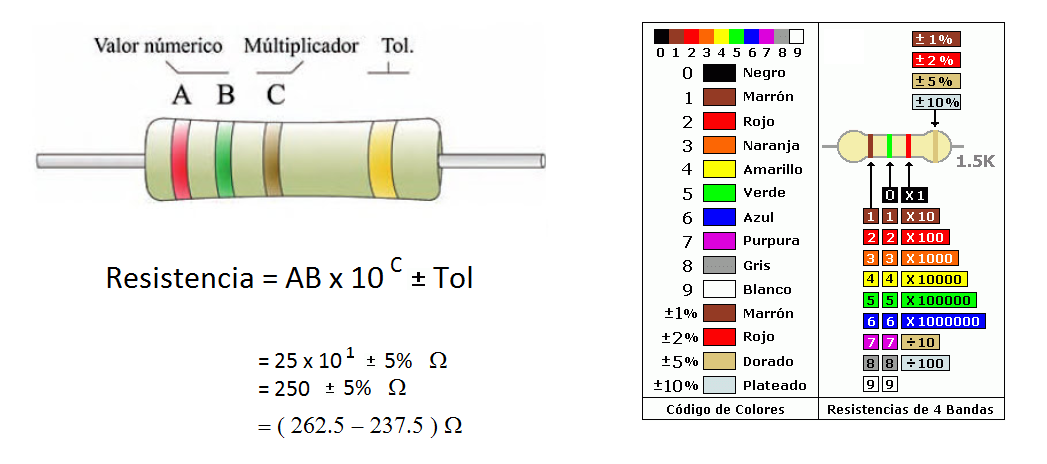
\includegraphics[width=0.8\textwidth]{image09.png}
    \caption{Ejemplo de lectura de Resistencia.}
    \label{fig:colores}
\end{figure}

Otro componente que utilizaremos en la práctica será el diodo luminiscente LED, utilizado en gran
medida como señalizador de encendido en equipos electrónicos. El diodo presenta 2 terminales, el
ánodo y el cátodo: el ánodo físicamente presenta una patilla más larga y en su símbolo la patilla
se conecta a la base de un triángulo; en el terminal del cátodo se ha diseñado el LED con un
pequeño aplanamiento y el símbolo de la patilla presenta una raya. Esto se puede apreciar en la
figura~\ref{fig:led}. Para que funcione un LED se debe aplicar por lo menos entre
$(1{,}5 - 2{,}2)$~V y una corriente comprendida entre $(10 - 50)$~mA.

\begin{figure}[H]
    \centering
    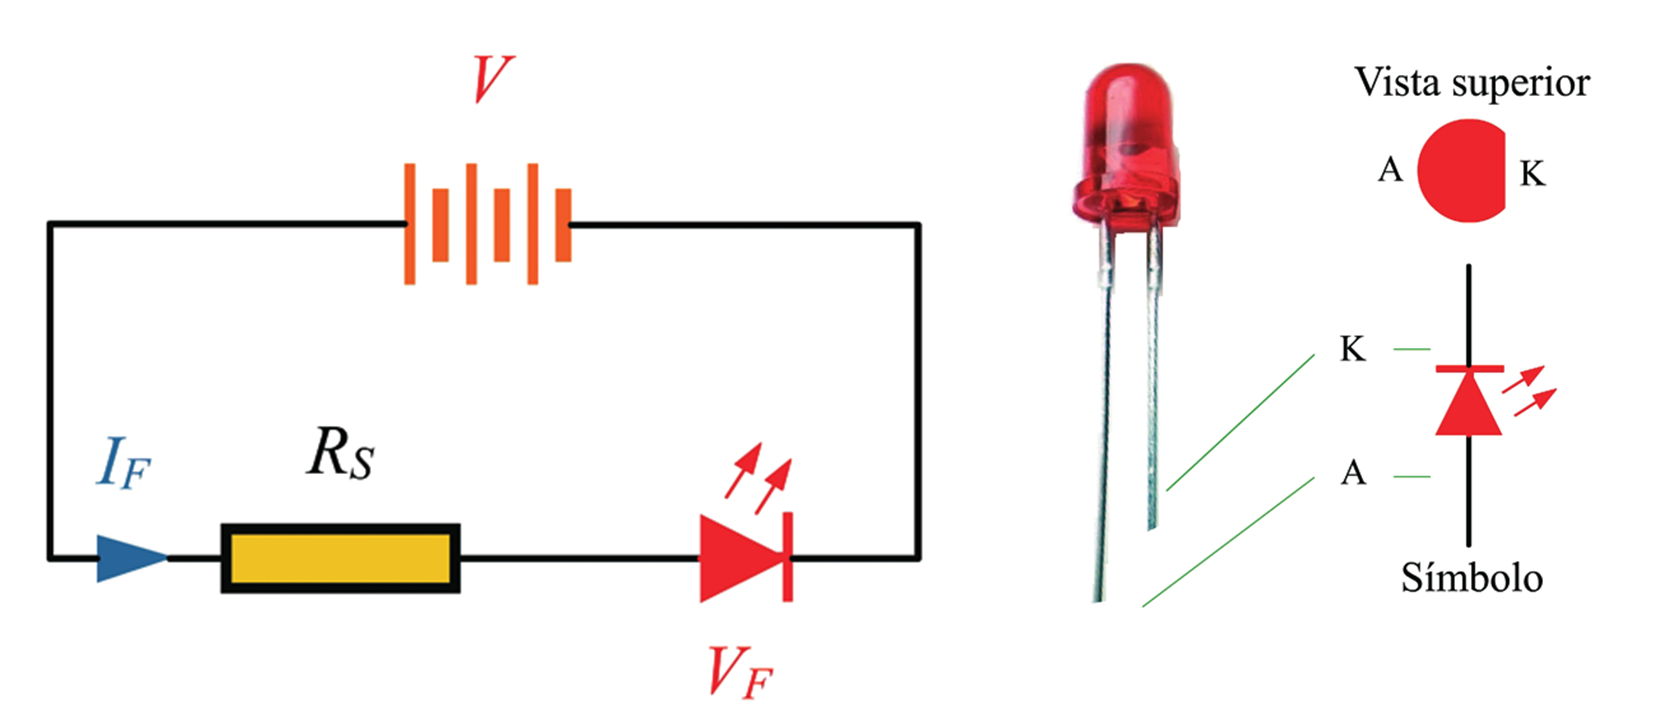
\includegraphics[width=0.85\textwidth]{image10.png}
    \caption{Símbolo y conexionado de un diodo LED.}
    \label{fig:led}
\end{figure}

Finalmente tocaremos el tema del \emph{Protoboard} o placa de montaje rápido. Estas placas poseen
una serie de orificios interconectados entre sí, como se muestra en la figura~\ref{fig:proto}, en
donde se pueden conectar los dispositivos electrónicos y se pueden realizar todo tipo de
circuitos; las filas superiores e inferiores se suelen utilizar para conectar la tensión de
alimentación del circuito.

\begin{figure}[H]
    \centering
    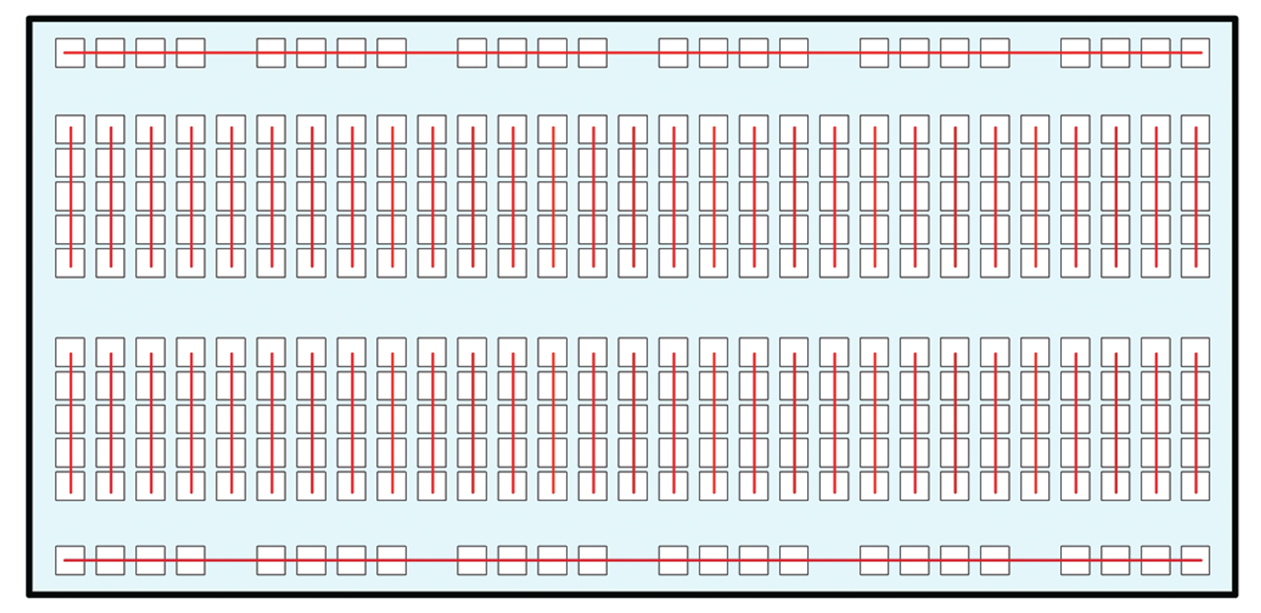
\includegraphics[width=0.8\textwidth]{image11.png}
    \caption{Esquema de conexionado de una placa Protoboard.}
    \label{fig:proto}
\end{figure}

%=======================================================================
\section*{III.\quad Cuestionario previo}

\begin{enumerate}
\item Complete la siguiente Tabla usando la ley de Ohm.

\begin{table}[H]
    \centering
    \renewcommand{\arraystretch}{1.4}
    \begin{tabular}{|c|c|c|c|}
    \hline
    \textbf{Ejercicio} & \textbf{I} & \textbf{V} & \textbf{R}\\
    \hline
    1 & 1 A      & 5 V    & \\
    \hline
    2 & 2 A      &        & 5 k$\Omega$\\
    \hline
    3 & 300 mA   & 20 mV  & \\
    \hline
    4 &          & 1 kV   & 10 k$\Omega$\\
    \hline
    5 &          & 5 V    & 330 $\Omega$\\
    \hline
    \end{tabular}
\end{table}

\item Escoja 4 resistencias diferentes y complete la siguiente tabla.

\begin{table}[H]
    \centering
    \footnotesize
    \renewcommand{\arraystretch}{1.6}
    \begin{tabular}{|c|c|c|c|c|c|c|c|}
    \hline
    \textbf{Ejercicio} & \textbf{Color 1} & \textbf{Color 2} & \textbf{Color 3} &
    \textbf{Color 4} & \textbf{\parbox{1.6cm}{\centering Valor de Resistencia}} &
    \textbf{Tolerancia} & \textbf{\parbox{2.2cm}{\centering Resistencia (Máx. -- Mín.)}}\\
    \hline
    1 & & & & & & & \\
    \hline
    2 & & & & & & & \\
    \hline
    3 & & & & & & & \\
    \hline
    4 & & & & & & & \\
    \hline
    \end{tabular}
\end{table}

\item Describa con sus propias palabras qué es una bocina y cómo funciona.

\vspace{0.4cm}
\linearesp
\linearesp
\linearesp
\end{enumerate}

%=======================================================================
\section*{IV.\quad Equipos y materiales}

\noindent\textbf{Laboratorio:} Electrónica y Comunicaciones.

\vspace{0.3cm}
\noindent\textbf{Equipos y dispositivos:}
\begin{itemize}
    \item 1 Computador Personal
    \item 1 EEB
    \item 1 Diodo LED
    \item 2 resistencias
    \item 1 potenciómetro
    \item 1 bocina
\end{itemize}

\noindent\textbf{Software:}
\begin{itemize}
    \item WaveForms 2015
\end{itemize}

%=======================================================================
\section*{V.\quad Actividades}

\subsection*{1.\quad Actividad: Conectando la Electronics Explorer Board}

\begin{itemize}
\item La \emph{Electronics Explorer Board} es un sistema de medición todo en uno, que sirve para
diseñar y probar circuitos analógicos y digitales. Está construida en base a 2 placas protoboard,
y permite el prototipado rápido y simple de circuitos. La operación de la EE Board es fácil de
manejar a través del software WaveForms de Digilent; los componentes de la tarjeta se pueden
observar en la figura~\ref{fig:eeb}.
\end{itemize}

\begin{figure}[H]
    \centering
    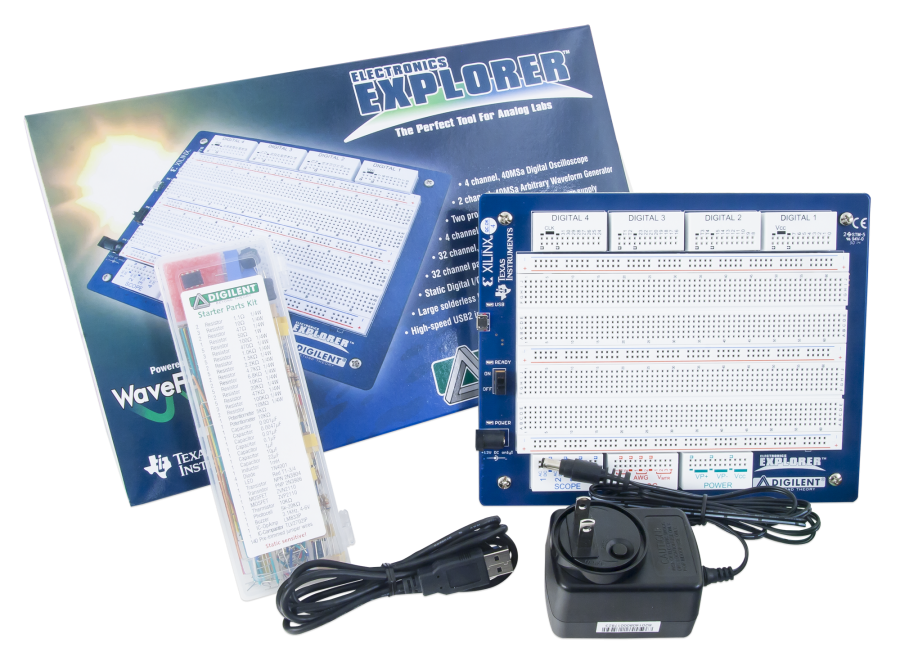
\includegraphics[width=0.75\textwidth]{image12.png}
    \caption{Componentes de la tarjeta EE Board.}
    \label{fig:eeb}
\end{figure}

\begin{itemize}
\item La comunicación con la EE Board se realiza a través de una conexión USB y la interconexión
es bastante simple. Se utiliza un cable micro-USB para conectar la tarjeta a un ordenador. La EE
Board también tiene un adaptador de jack de alimentación de 12~V de energía externa. Con el cable
USB y la fuente de alimentación externa conectada, girar el interruptor de la tarjeta a
\textbf{ON}, lo cual prepara a la EE Board para la comunicación con el software WaveForms. Esta
conexión se puede apreciar en la figura~\ref{fig:conex}.
\end{itemize}

\begin{figure}[H]
    \centering
    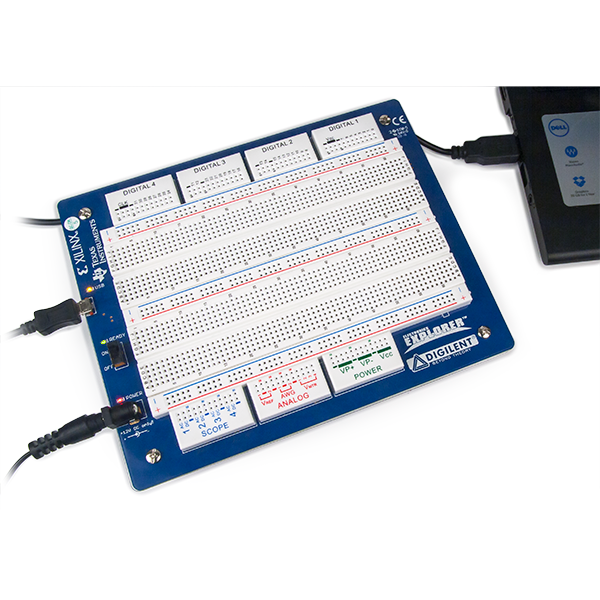
\includegraphics[width=0.55\textwidth]{image13.png}
    \caption{Conexionado de la tarjeta EE Board.}
    \label{fig:conex}
\end{figure}

\begin{itemize}
\item Las partes que conforman la tarjeta se pueden separar en 3 grupos, que son: la zona de
instrumentos, la tarjeta protoboard o \emph{breadboard} y la zona de conexiones digitales. Esto
se aprecia en la figura~\ref{fig:grupos}.
\end{itemize}

\begin{figure}[H]
    \centering
    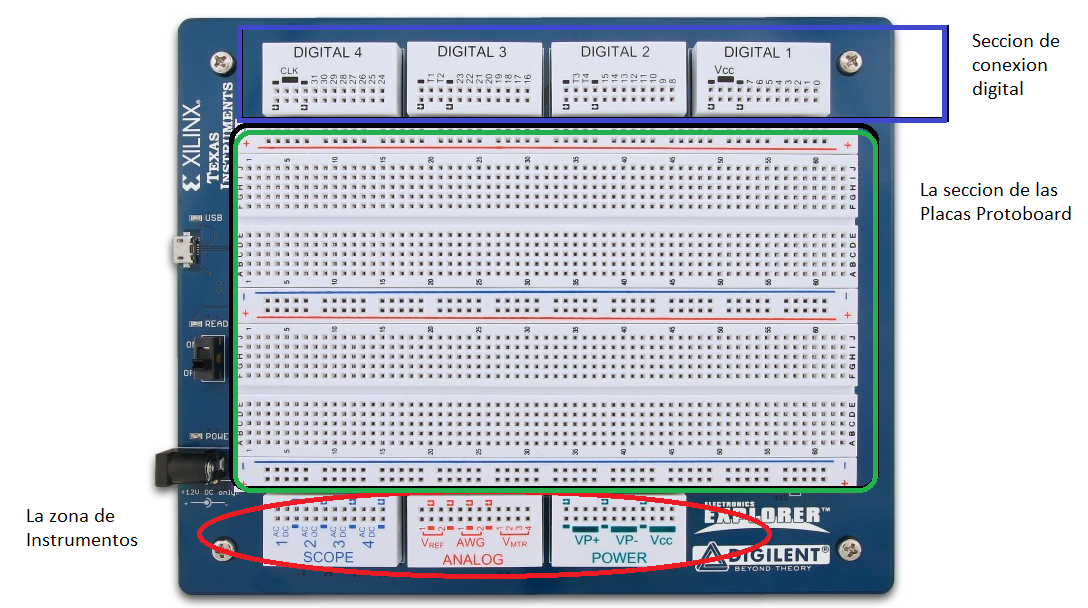
\includegraphics[width=0.8\textwidth]{image14.png}
    \caption{Grupo de partes que conforman la tarjeta EE Board.}
    \label{fig:grupos}
\end{figure}

\noindent Específicamente, la EE Board cuenta con:

\begin{itemize}
\item \textbf{4 canales de Osciloscopio a 40~MS/s, 100~MHz.}

    \begin{minipage}[c]{0.30\textwidth}
        \centering
        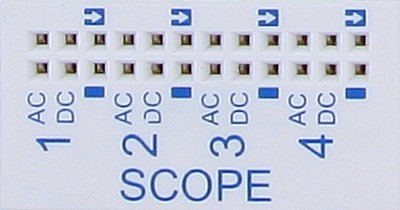
\includegraphics[width=\linewidth]{image15.png}
    \end{minipage}
    \hfill
    \begin{minipage}[c]{0.62\textwidth}
        Dónde:
        \begin{itemize}
            \item \textbf{AC}: canal sin offset de voltaje.
            \item \textbf{DC}: canal con offset de voltaje.
            \item \textbf{--}: es la tierra.
        \end{itemize}
    \end{minipage}

\vspace{0.4cm}

\item \textbf{2 canales, 40~MS/s, 20~MHz, generador de forma de onda arbitraria.}

    \begin{minipage}[c]{0.30\textwidth}
        \centering
        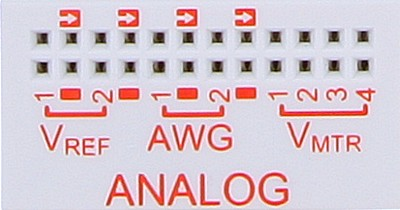
\includegraphics[width=\linewidth]{image16.png}
    \end{minipage}
    \hfill
    \begin{minipage}[c]{0.62\textwidth}
        Dónde:
        \begin{itemize}
            \item \textbf{AWG 1}: primer canal.
            \item \textbf{AWG 2}: segundo canal.
            \item \textbf{--}: es la tierra.
        \end{itemize}
    \end{minipage}

\vspace{0.4cm}

\item \textbf{4 canales de Voltímetro (VMTR).}

\item \textbf{2 voltajes de referencia programables:} VREF~1 y VREF~2.

\vspace{0.2cm}

\item \textbf{2 canales, $\pm$9~V, 1,5~A, fuente de alimentación variable.}

    \begin{minipage}[c]{0.30\textwidth}
        \centering
        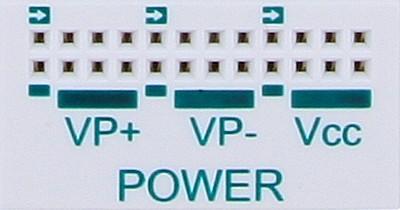
\includegraphics[width=\linewidth]{image17.png}
    \end{minipage}
    \hfill
    \begin{minipage}[c]{0.62\textwidth}
        Dónde:
        \begin{itemize}
            \item \textbf{VP+}: es $+9$~V, 1,5~A.
            \item \textbf{VP--}: es $-9$~V, 1,5~A.
            \item \textbf{--}: es la tierra.
        \end{itemize}
    \end{minipage}

\vspace{0.4cm}

\item \textbf{1 canal, 3.3~/~5~V, 2~A, fuente de alimentación fija (Vcc).}

\item \textbf{Puede conectar 32 señales digitales} que se pueden configurar como:
    \begin{itemize}
        \item Analizador lógico de 32 canales.
        \item Generador de patrones de 32 canales.
        \item E/S digitales discretas (botones, interruptores, LEDs, etc.).
    \end{itemize}
\end{itemize}

\begin{figure}[H]
    \centering
    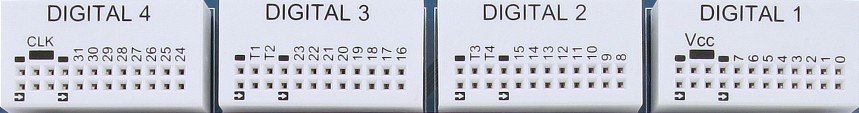
\includegraphics[width=0.9\textwidth]{image18.png}
    \caption{Zona de conexiones digitales de la EE Board.}
    \label{fig:digital}
\end{figure}

\begin{itemize}
\item En cuanto al software WaveForms, antes de iniciarlo conecte la EE Board al ordenador,
conecte su transformador y encienda el switch (ON); después ejecute el programa y le aparecerá
la imagen de la figura~\ref{fig:waveforms}. Acepte la configuración por defecto de la EE Board.
\end{itemize}

\begin{figure}[H]
    \centering
    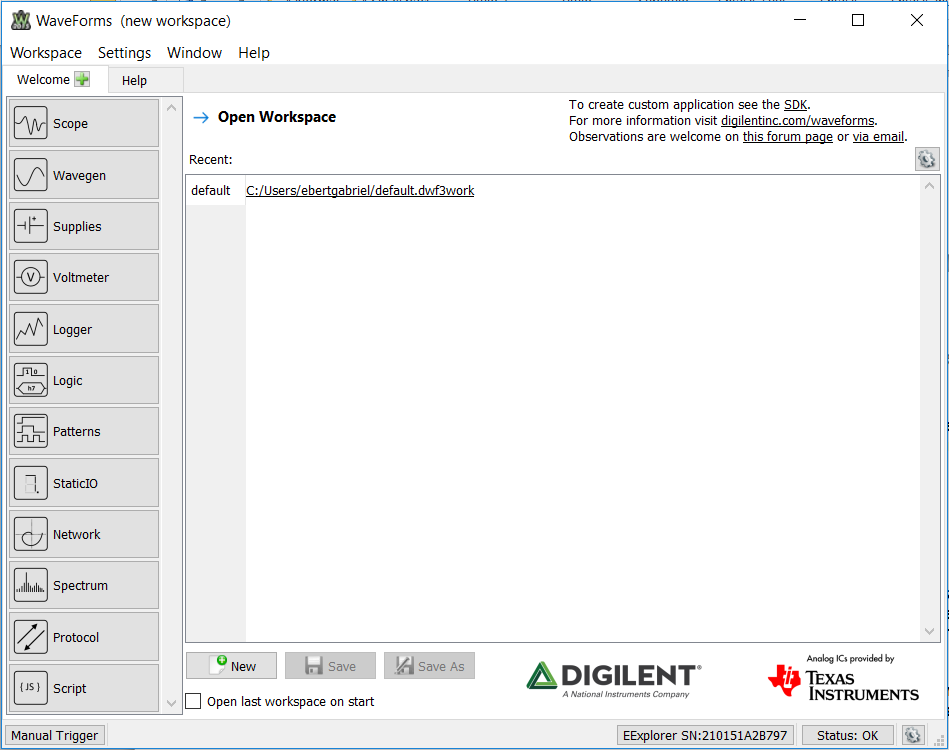
\includegraphics[width=0.7\textwidth]{image19.png}
    \caption{Pantalla de Inicio del Software WaveForms.}
    \label{fig:waveforms}
\end{figure}

\subsection*{2.\quad Actividad: Mi primer circuito}

\begin{itemize}
\item En este primer circuito haremos simplemente un circuito serie que nos permitirá encender y
apagar un diodo LED. Para esto arme en la zona protoboard de la EE Board el circuito esquemático
mostrado en la figura~\ref{fig:esquema}; para tener una mejor perspectiva del circuito puede
revisar la figura~\ref{fig:implement}.
\end{itemize}

\begin{figure}[H]
    \centering
    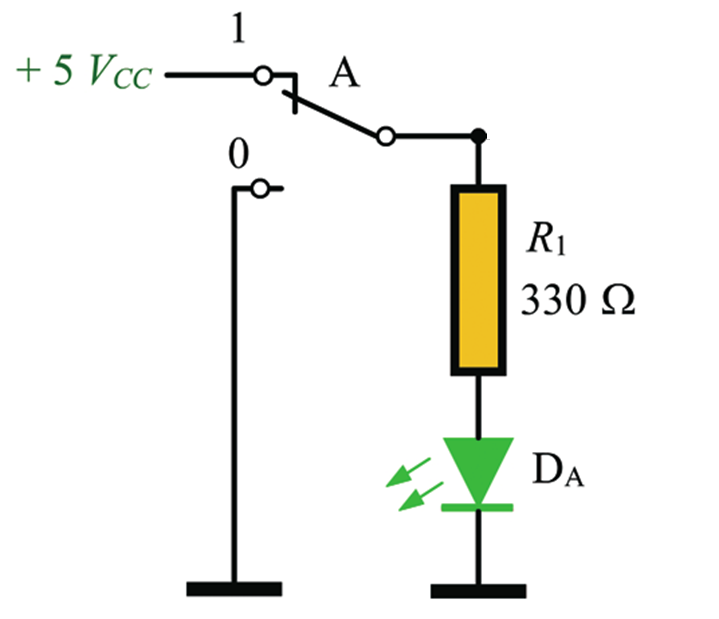
\includegraphics[width=0.5\textwidth]{image20.png}
    \caption{Esquemático del circuito a implementar.}
    \label{fig:esquema}
\end{figure}

\begin{itemize}
\item Configure el circuito de la figura~\ref{fig:implement} y tenga cuidado con las patillas de
conexión del LED; después configure el software, en la opción \emph{Static I/O} cambie el tipo de
switch y pruebe que el LED enciende. Esto se puede apreciar en la figura~\ref{fig:switch}.
\end{itemize}

\begin{figure}[H]
    \centering
    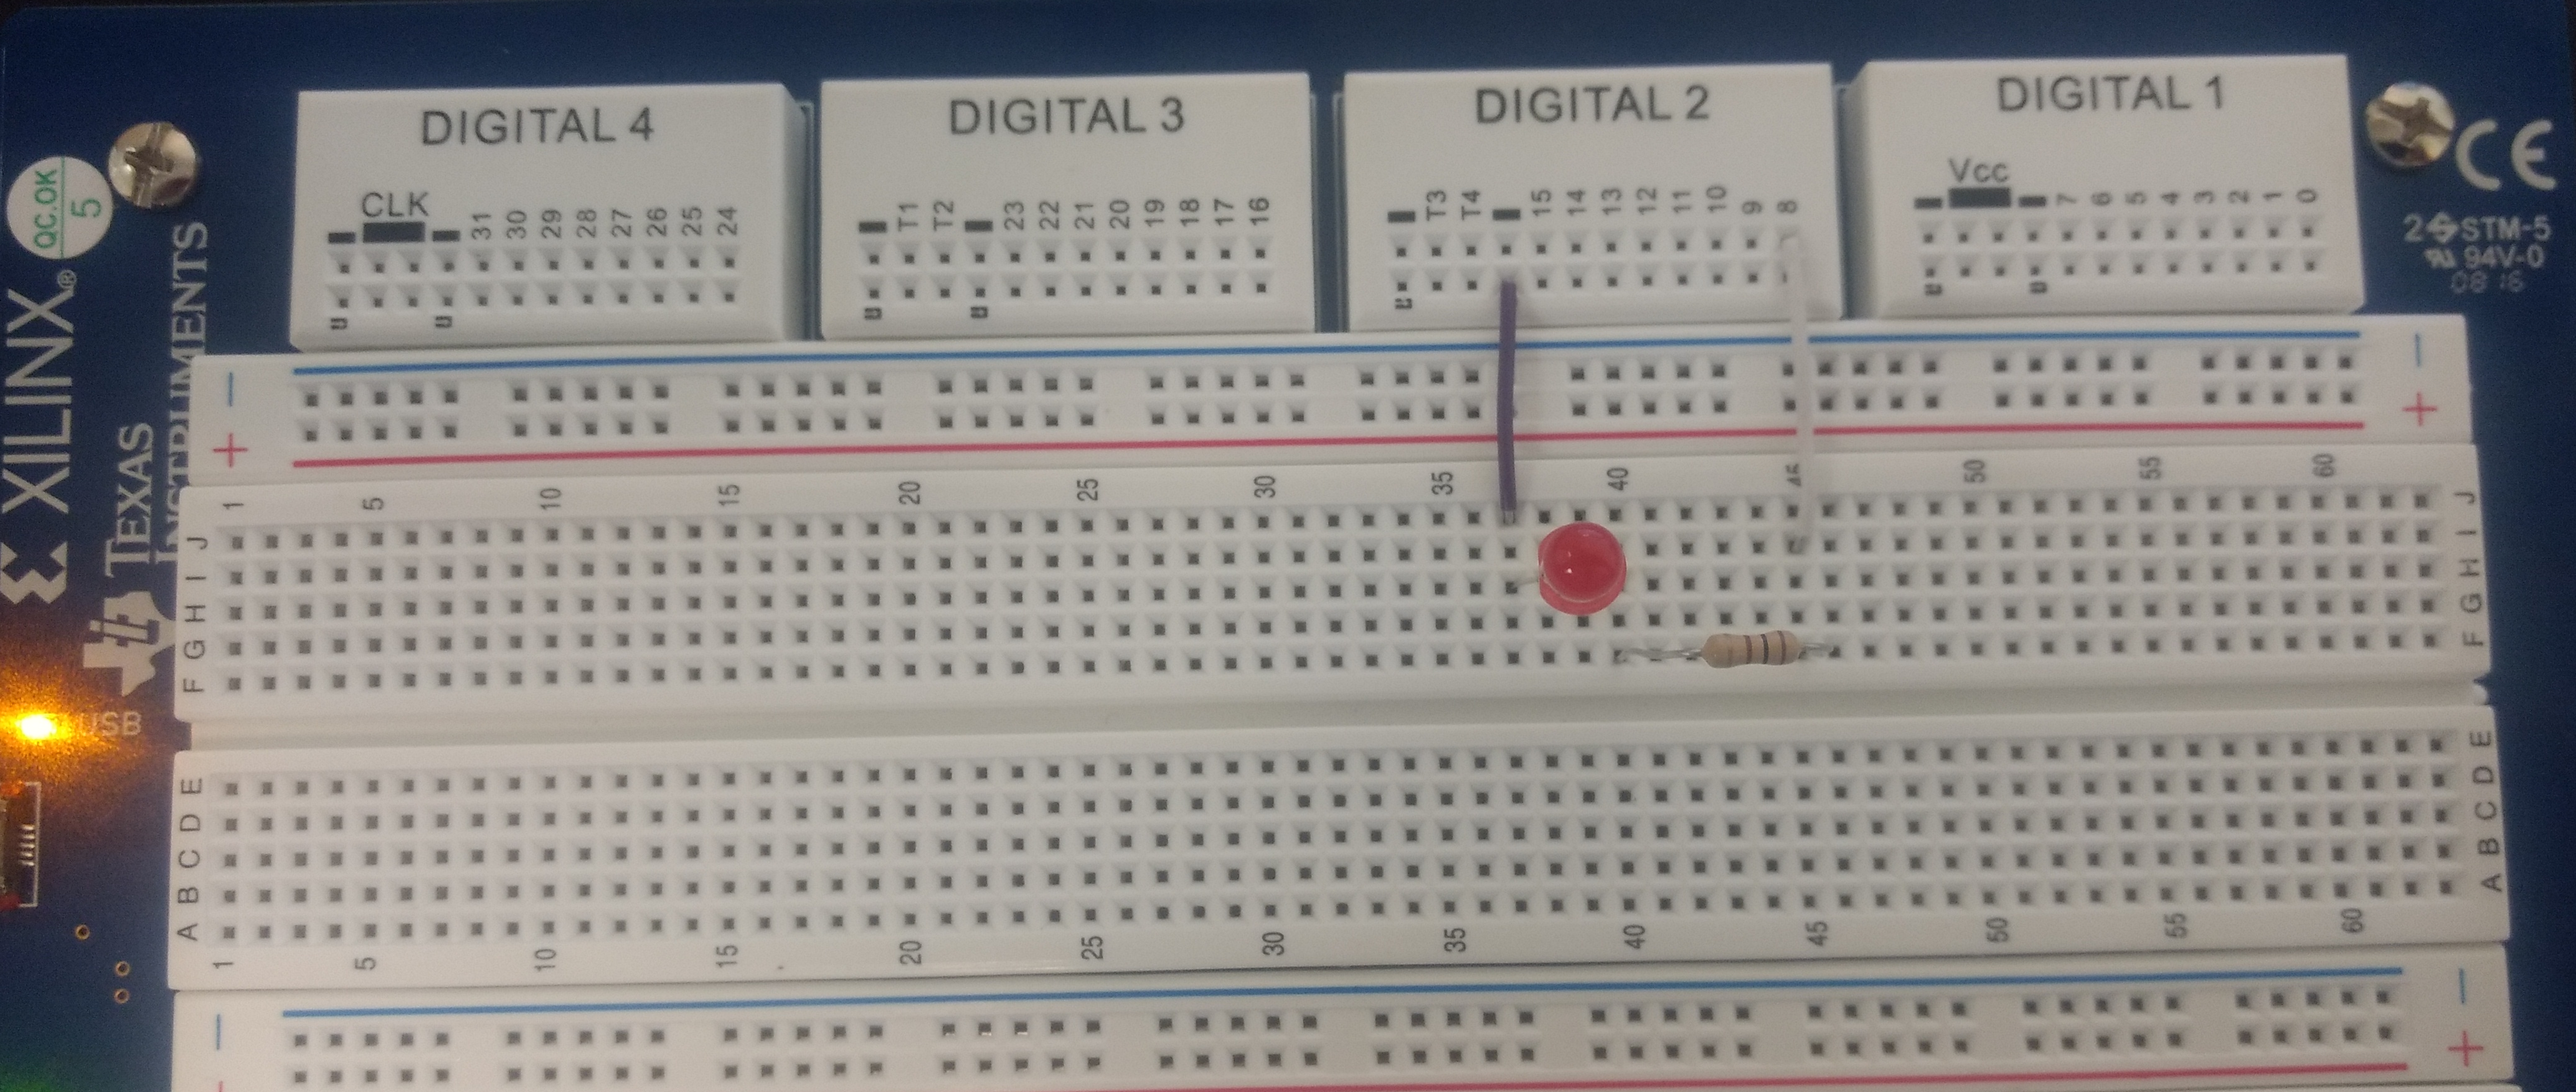
\includegraphics[width=\textwidth]{image21.png}
    \caption{Implementación del circuito en la EE Board.}
    \label{fig:implement}
\end{figure}

\begin{figure}[H]
    \centering
    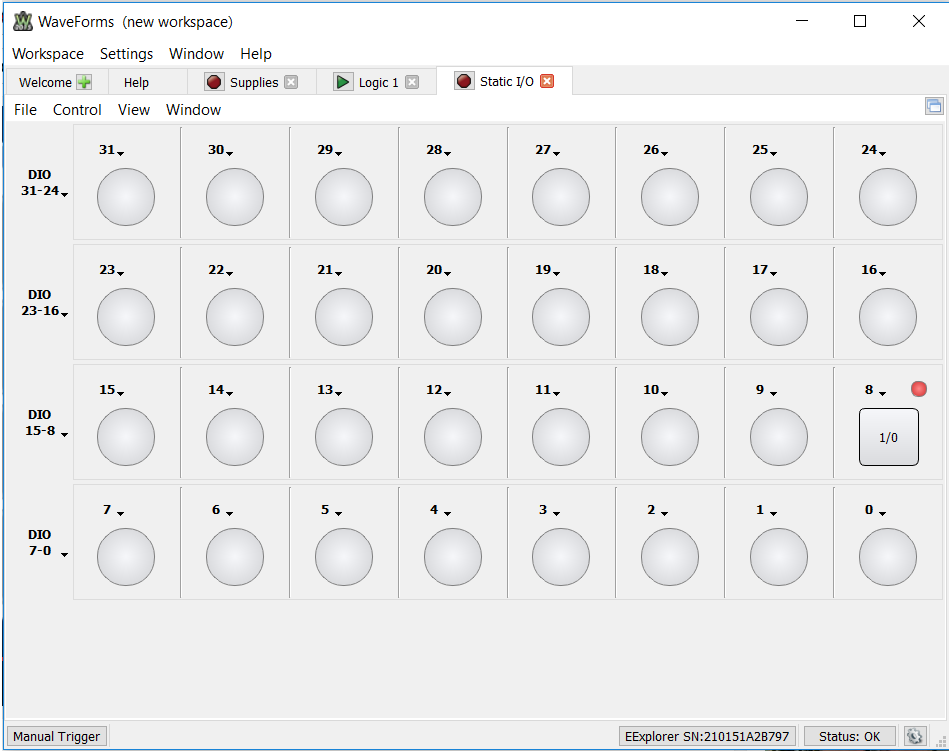
\includegraphics[width=0.7\textwidth]{image22.png}
    \caption{Configuración del switch en el software WaveForms.}
    \label{fig:switch}
\end{figure}

%=======================================================================
\section*{VI.\quad Tarea asignada}

\begin{itemize}
    \item Ninguna, es un Taller.
\end{itemize}

\end{document}
